%%
%% This is file `thesis.tex',
%% generated with the docstrip utility.
%%
%% The original source files were:
%%
%% scnuthesis.dtx  (with options: `thesis')
%% 
%% This is a generated file.
%% 
%% Copyright (C) 2013 by Joseph Pan <cs.wzpan@gmail.com>
%% 
%% This file may be distributed and/or modified under the
%% conditions of the LaTeX Project Public License, either version 1.3a
%% of this license or (at your option) any later version.
%% The latest version of this license is in:
%% 
%% http://www.latex-project.org/lppl.txt
%% 
%% and version 1.3a or later is part of all distributions of LaTeX
%% version 2004/10/01 or later.
%% 
%% To produce the documentation run the original source files ending with `.dtx'
%% through LaTeX.
%% 
%% Any Suggestions : LiuBenYuan <liubenyuan@gmail.com>
%% Thanks Xue Ruini <xueruini@gmail.com> for the thuthesis class!
%% Thanks sofoot for the original NUDT paper class!
%% 
%1. 如果是研究生论文,常用的选项是:
% \documentclass[master,twoside,ttf]{scnuthesis}
%2. 如果是博士生论文,常用的选项是:
% \documentclass[doctor,twoside,ttf]{scnuthesis}
%3. 如果使用是Vista、Windows 7或者使用从Vista或Windows 7拷贝过来的字体,则需要再加一个Vista选项,如:
% \documentclass[master,twoside,ttf,vista]{scnuthesis}
%4. 建议使用OTF字体获得较好的页面显示效果
%   OTF字体从网上获得,各个系统名称统一,不用加vista选项
%   如果你下载的是最新的(1201)OTF英文字体,建议修改scnuthesis.cls,使用PS Std
%   \documentclass[doctor,twoside,otf]{scnuthesis}
%5. 如果想生成盲评,传递anon即可,仍需修改个人成果部分
% \documentclass[master,otf,anon]{scnuthesis}
%6. 让章节标题作为页眉,可以使用chapterhead选项。如果和twoside一起使
% \documentclass[master,otf,twoside,chapterhead]{scnuthesis}
%
\documentclass[master,twoside,ttf,chapterhead]{scnuthesis}
\usepackage{myscnu}

\begin{document}
\graphicspath{{figures/}}
\classification{}
\university{10574}
\confidentiality{无}
\serialno{2011123456}
\title{华南师范大学硕士/博士\\
  学位论文\LaTeX{}模板使用手册}
\displaytitle{华南师范大学硕士/博士学位论文\LaTeX{}模板使用手册}
\author{张三}
\subject{计算机应用技术}
\researchfield{数字图像处理}
\school{计算机学院}
\supervisor{李四\quad{}教授}
\zhdate{\zhtoday}
\entitle{How to Use the \LaTeX{} Document Class for SCNU Dissertations}
% 插入摘要,制作封面
\ifisanon{}\else{\maketitle}\fi

\frontmatter

%!TEX root = ../thesis.tex
\begin{cabstract}
华南师范大学是一所有着悠久历史和深厚人文底蕴的高等学府,学校地处中国改革开放之%
都——广州,深得岭南开放务实之精神,有着素朴的传统和良好的学风,七十多年来,学校坚%
持师范教育的特色,始终致力于培养人格健全、有思想、有能力、有社会责任感的优秀人才。%

在大学日益参与经济社会发展的新世纪,华南师范大学正以崭新的风貌、开阔的世界眼光,%
不断拓展大学的育人理念,创造良好的教学和包容的学术研究环境,营造丰富的校园文化,%
努力构建特色鲜明、开放式、综合性高水平教学研究型大学。%
\end{cabstract}
\ckeywords{华南师范大学;论文;模板}

\begin{eabstract}
  South China Normal University is an institution of higher education with a
  long history and a rich legacy. Situated in Guangzhou, the open metropolis in
  South China, South China Normal University is imbued with Lingnan's
  pioneering and pragmatic spirits. It has developed a tradition of elegant
  simplicity and fostered a strong learning environment. In the past seventy
  years or so, South China Normal University has preserved its characteristics
  of teacher education and has been devoted to cultivating talents with moral
  integrity, independent thinking, innovative ability and sense of social
  responsibility.

  In the new century in which the institutions of higher education are getting
  increasingly involved in the social and economic development, South China
  Normal University has adopted an international view on education. Having
  broadened its horizon on the key issue of cultivating talents, it has made its
  greatest efforts to create a congenial and harmonious environment for both
  teaching and academic research and has fostered a rich variety of campus
  culture. It aims to build itself into a high-level comprehensive teaching and
  research-oriented university with open distinctive features.
\end{eabstract}
\ekeywords{SCNU; thesis; template}


% 生成目录
\tableofcontents
\listoftables           % 如果要生成表目录
\listoffigures          % 如果要生成图目录

\renewcommand{\chapterlabel}{\denotationname} %设置页眉

\begin{denotation}

\item[SCNU] 华南师范大学 (South China Normal University)
\item[API] 应用程序编程接口  
\item[cluster] 集群
\item[graphic] 图形
\item[communication] 通信
\item[3D] 三维 (Three Dimemsion)
\item[BMP] 位图
\item[PNG] 便携式网络图形 (Portable Network Graphics)
\item[Watershed] 分水岭
\item[GUI] 图形用户界面 (Graphical User Interface)
\item[$E$] 能量
\item[$m$] 质量
\item[$c$] 光速
\item[$P$] 概率
\item[$T$] 时间
\item[$v$] 速度

\end{denotation}
 % 如果要生成符号列表

\mainmatter
\pagestyle{mpage}
\chapter{绪论}

\section{本模板的意义}

\subsection{现有的学位论文模板的不足}
学位论文作为高校教学计划中的重要环节,对提高教学质量、培养学生综合应用能力具有十%
分重要的意义。根据国家制定的《科学技术报告、学位论文和学术论文的编写格式》,华南%
师范大学采用Microsoft Word等文字处理系统制作了相应的学位论文模板。然而,在应用这%
些模板的过程中,却出现了几下几种问题\cite{Maddage2009}:
\begin{enumerate}
\item 无法自动处理图表、公式的序号、参考文献引用标号的变动,经常出现因疏忽而前后%
  文体格式不一致的现象;
\item 无法实现论文的格式和内容的有效分离,导致模板的格式很容易被学生无意中修改,%
  从而影响了学位论文规范化管理的质量;
\item 受制于Word版本的兼容性问题,在不同版本的文档之间常会有显示上的出入。%
\end{enumerate}

\subsection{\LaTeX{}的特性}
\TeX{}作为一个功能强大的特别适合于排版科技文献和书籍的格式化排版程序~,其具有以下几点特性:
\begin{enumerate}
\item 强大的宏定义功能。\TeX{}是一种宏命令编程语言,能够处理非常复杂的排版任务,并生成高质量的输出;
\item 方便的自动编号功能。文章、书籍的章、节、段落以及公式、图表、参考文献、页码等均可自动编号;
\item 良好的通用性。\LaTeX{}几乎在所有的计算机操作系统平台上得到实现。\LaTeX{}的源文%
  件可在不同的平台之间自由的交换,而得到的输出是完全相同的。
\end{enumerate}




\subsection{采用\LaTeX{}学位论文模板的意义}
采用\LaTeX{}学位论文模板将有以下几点意义:
\begin{enumerate}
\item 有效地解决以往的\verb|Word|模板中所存在的问题,有助于提高毕业生的学位论文的排版质量;
\item 有助于推动LaTeX在学生群体中的普及,学会使用\LaTeX{}来生成高质量的文档;
\item 本模板在Github\footnote{项目主页:
    \url{http://github.com/wzpan/scnuthesis/}}上开源。让更多爱好者研究学习,并不断完善,以适应日后的需求。
\end{enumerate}


\section{(1.2 题目)}
绪论内容

绪论内容

绪论内容

绪论内容

绪论内容

绪论内容

\section{(1.3 题目)}
绪论内容

绪论内容

绪论内容

绪论内容

绪论内容

绪论内容

\subsection{(1.3.1 题目)}
绪论内容

绪论内容

绪论内容

绪论内容

\subsection{(1.3.2 题目)}

绪论内容

绪论内容



%!TEX root = ../thesis.tex
\chapter{论文正文}
\label{chap:main}
本章将进入论文排版的正文
主要包括:字体段落,图片表格,公式定理,参考文献四部分。
版面将包括在\scnuthesis{}中使用到的所有格式,模板中自定义命令到或者特有的东西都将被一一介绍,
希望大家能看到对自己有用的东西,方便上手。

为了节省时间,这份说明的内容同样参考了国防科技大学的\nudtpaper{}模板~,在此表示感谢。

\section{字体段落}
\label{sec:font}

本节内容来自华南师范大学外部门户\footnote{外部门户主页:\url{http://www.scnu.edu.cn/}}。

华南师范大学始建于1933年,是一所学科门类齐全的国家“211 工程”重点建设大学和广东%
省省属重点大学。学校现有广州石牌、广州大学城和南海3个校区,占地面积共3079亩,%
校舍面积共 126万平方米。校园环境优美,景色怡人~,人文景观遍布,文化气息浓厚,为广%
大师生提供了良好的学习、工作和生活环境。

学校现有4个国家重点学科(含1个重点培育学科), 9个国家“211 工程”重点建设学%
科,2个广东省一级学科重点学科,11个广东省二级学科重点学科。有71个本科专业,有14个%
博士学位授权一级学科、90个博士学位授权点(未含2011年8月一级学科调整后新增的博士%
点)、1个博士专业学位授权点,33个硕士学位授权一级学科、174个硕士学位授权点(未%
含2011年8月一级学科调整后新增的硕士点)、10个硕士专业学位授权点,涉及到哲学、经济%
学、法学、教育学、文学、历史学、理学、工学、管理学、农学、医学等11个学科门%
类。 有12个博士后流动站。

学校拥有一批实力较强的实验室和科研基地。有教育部激光生命科学重点实验室、环境理论
化学重点实验室(省部共建)、教育部电化学储能材料与技术工程研究中心、卫生部(中医
药管理局)中医药与光子技术实验室、国家理科基础科学研究和教学人才培养基地、教育部
部省共建人文社科重点研究基地(心理应用研究中心)、国家体育总局重点研究基地(体育
社会科学研究基地),有7个广东省重点实验室(中心),6个广东省高校科研型重点实验
室,3个广东省高校产学研结合示范基地,6个广东省普通高校人文社会科学重点研究基
地,1个广东省高校工程技术研究中心。学校还拥有“物理学科基础课”、“信息传
播”~、“心理学”等3个国家级实验教学示范中心,7个广东省实验教学示范中心。此外,教
育部高校辅导员培训和研修基地、广东省普通高等学校师资培训中心~、广东省网络图书馆、
广东高校建筑规划设计院等机构均设在学校。

70 多年来,学校数易校名,几度迁徙,虽历经沧桑,却弦歌不辍。一代又一代华师人秉承勷
勤大学师范学院{\kai “研究高深学术,养成社会之专门人才”}的优良传统,承传南方大
学{\kai “忠诚团结,朴实虚心,勤劳勇敢,实事求是”}的革命精神~,践行{\kai “艰苦奋斗、严谨治
学、求实创新、为人师表”}的校训,筚路蓝缕,薪火相传,共同铸就了学校今天的繁荣与
发展。

华南师范大学历史上的名字包括:

\begin{itemize}
\item[楷体] {\kai 广州市立师范学校}
\item[黑体] {\hei 勷勤大学师范学院}
\item[隶书] {\li 勷勤大学教育学院}
\item[宋体] {\song 广东省立教育学院}
\item[仿宋] {\fs 广东省立文理学院}
\item[粗体] {\bfseries 广东省文理学院}
\item[斜体] {\itshape 华南师范学院}
\item[粗斜体] {\bfseries\itshape 广东师范学院}
\item[字体颜色] {\textcolor{red}{华南师范大学}}
\end{itemize}

上面这段内容使用了itemize列表环境,\LaTeX{}默认的列表环境会在条目之间插入
过多的行距,若用户需要紧凑的行距,可以使用compactitem环境。

下面测试英文字体:

Remember the \textsf{more} \textbf{font} {\bfseries\tiny you \sffamily use,
\Large the \scshape more \itshape beautiful \slshape your \footnotesize
document becomes.}

\begin{itemize}
\item[英文黑体] Typeset text in \textbf{bold} series
\item[英文斜体] Typeset text in \textit{italic} shape
\item[Roman字体] Typeset text in roman family
\item[Sans Serif字体] Typeset text in \textsf{sans serif} family
\item[typewriter字体] Typeset text in \texttt{typewriter} family
\end{itemize}

下面测试字号:
\begin{itemize}
\item[初号] {\chuhao 华南师范大学}
\item[小初] {\xiaochu 华南师范大学}
\item[一号] {\yihao 华南师范大学}
\item[小一] {\xiaoyi 华南师范大学}
\item[二号] {\erhao 华南师范大学}
\item[小二] {\xiaoer 华南师范大学}
\item[三号] {\sanhao 华南师范大学}
\item[小三] {\xiaosan 华南师范大学}
\item[四号] {\sihao 华南师范大学}
\item[小四] {\xiaosi 华南师范大学}
\item[五号] {\wuhao 华南师范大学}
\item[小五] {\xiaowu 华南师范大学}
\end{itemize}

\section{表格明细}
\label{sec:figure}
表格是书中的重要组成部分,这一章将从简单的表格讲起,到复杂的表格为止。

\subsection{基本表格}
\label{sec:basictable}

模板中关于表格的宏包有三个: \textsf{booktabs}、\textsf{array} 和
\textsf{longtabular},命令有一个 \verb|\hlinewd|。三线表建议使用\textsf{booktabs}中提供的,
包含toprule、midrule 和 bottomrule三条命令。
它们与\textsf{longtable} 能很好的配合使用。如果表格比较简单的话可以直接用命令
\verb|hlinewd{xpt}| 控制。下面来看一个表格:
\begin{table}[htb]
  \centering
  \begin{minipage}[t]{0.8\linewidth} % 如果想在表格中使用脚注,minipage是个不错的办法
  \caption[模板文件]{模板文件。如果表格的标题很长,那么在表格索引中就会很不美
    观,所以要像 chapter 那样在前面用中括号写一个简短的标题。这个标题会出现在索
    引中。}
  \label{tab:template-files}
    \begin{tabular*}{\linewidth}{lp{10cm}}
      \toprule[1.5pt]
      {\hei 文件名} & {\hei 描述} \\
      \midrule[1pt]
      scnuthesis.ins & \LaTeX{} 安装文件,docstrip\footnote{表格中的脚注} \\
      scnuthesis.dtx & 所有的一切都在这里面\footnote{再来一个}。\\
      scnuthesis.cls & 模板类文件。\\
      scnuthesis.cfg & 模板配置文。cls 和 cfg 由前两个文件生成。\\
      bstutf8.bst   & 参考文献 Bibtex 样式文件。\\
      myscnu.sty    & 常用的包和命令写在这里,减轻主文件的负担。\\
      \bottomrule[1.5pt]
    \end{tabular*}
  \end{minipage}
\end{table}

如果你不需要在表格中插入脚注,可以将minipage环境去掉。

表 \ref{tab:template-files} 列举了本模板主要文件及其功能。
请大家注意三线表中各条线对应的命令。这个例子还展示了如何在表格中正确使用脚注。
由于 \LaTeX{} 本身不支持在表格中使用 \verb|\footnote|,所以我们不得不将表格放在
小页中,而且最好将表格的宽度设置为小页的宽度,这样脚注看起来才更美观。

如果遇到表格内容自动调整的问题,可以有两种解决办法: 其一就是用\verb|tabular*|,在
两列之间全部插入空白,该方法存在的缺点是当只有两列需要自动调整时,若小页预留空间
过大,可能插入过多的\verb|fill|,导致不美观; 另外一种就是使用\verb|tabularx|自动
调整了,需要定制一个\textbf{Z}环境,在新版本中,该命令已添加到\verb|myscnu.sty|中。
下面是这两个方法实现的对比,各位可以仔细对比一下,推荐使用后者。

\begin{table}[htbp]
\centering
\begin{minipage}[t]{0.9\linewidth}
\caption{Reed Solomon码的典型应用}
\label{tab:RSused}
\begin{tabular*}{\linewidth}{c @{\extracolsep{\fill}} c}
\toprule[1.5pt]
{\hei 应用领域} & {\hei 编码方案}\\
\midrule[1pt]
磁盘驱动器 & RS(32,28,5)码 \footnote{码长为32、维数为28、最小距离为5} \\
CD & 交叉交织RS码(CIRC) \\
DVD & RS(208,192,17)码、RS(182,172,11)码 \\
光纤通信 & RS(255,229,17)码 \\
\bottomrule[1.5pt]
\end{tabular*}
\end{minipage}
\end{table}

\begin{table}[htbp]
\centering
\begin{minipage}[t]{0.9\linewidth}
\caption{Reed Solomon码的典型应用}
\label{tab:RSuse}
\begin{tabularx}{\linewidth}{cZ}
\toprule[1.5pt]
{\hei 应用领域} & {\hei 编码方案}\\
\midrule[1pt]
磁盘驱动器 & RS(32,28,5)码 \footnote{码长为32、维数为28、最小距离为5} \\
CD & 交叉交织RS码(CIRC) \\
DVD & RS(208,192,17)码、RS(182,172,11)码 \\
光纤通信 & RS(255,229,17)码 \\
\bottomrule[1.5pt]
\end{tabularx}
\end{minipage}
\end{table}

\subsection{复杂表格}
\label{sec:complicatedtable}

我们经常会在表格下方标注数据来源,或者对表格里面的条目进行解释。前面的脚注是一种
不错的方法,如果你不喜欢脚注。那么完全可以在表格后面自己写注释,比如表~\ref{tab:tabexamp1}。
\begin{table}[htbp]
  \centering
  \caption{复杂表格示例 1}
  \label{tab:tabexamp1}
  \begin{minipage}[t]{0.8\textwidth} 
    \begin{tabularx}{\linewidth}{|l|X|X|X|X|}
      \hline
      \multirow{2}*{\backslashbox{x}{y}}  & \multicolumn{2}{c|}{First Half} & \multicolumn{2}{c|}{Second Half}\\
      \cline{2-5}
      & 1st Qtr &2nd Qtr&3rd Qtr&4th Qtr \\ 
      \hline
      East$^{*}$ &   20.4&   27.4&   90&     20.4 \\
      West$^{**}$ &   30.6 &   38.6 &   34.6 &  31.6 \\ 
      \hline
    \end{tabularx}\\[2pt]
    \footnotesize
    *:东部\\
    **:西部
  \end{minipage}
\end{table}

此外,表~\ref{tab:tabexamp1} 同时还演示了另外两个功能:1)通过 \textsf{tabularx} 的
 \texttt{|X|} 扩展实现表格自动放大;2)通过命令 \verb|\backslashbox| 在表头部分
插入反斜线。

为了使我们的例子更接近实际情况,我会在必要的时候插入一些“无关”文字,以免太多图
表同时出现,导致排版效果不太理想。

学校七十余载薪火相传,名师荟萃,著名的教育家罗浚、汪德亮,五四新诗开创者之一康白
情,古代文学家李镜池,古汉语学家吴三立,历史学家王越,逻辑学家李匡武,心理学家阮
镜清,教育学家叶佩华、朱勃,数学家叶述武,物理学家黄友谋、刘颂豪,著名体育教育家
袁浚等众多名家、名师先后在此执教。该校虽数度易名、几经迁徙,但一代又一代华师人秉
承勷勤大学师范学院``研究高深学术,养成社会之专门人才''的优良传统,承传南方大
学``忠诚团结,实事求是''的革命精神,践行``艰苦奋斗、严谨治学、求实创新、为人师
表''的校训,不断推动学校事业向前发展。特别是改革开放以来,抓住科教兴国、人才强国
的发展机遇,凭借建设文化省、教育强省和国家``211工程''的强劲东风,形成了学校现在
跨越式发展的大好局面。

不可否认 \LaTeX{} 的表格功能没有想象中的那么强大,不过只要你足够认真,足够细致,那么
同样可以排出来非常复杂非常漂亮的表格。请参看表~\ref{tab:tabexamp2}。
\begin{table}[htbp]
  \centering\dawu[1.3]
  \caption{复杂表格示例 2}
  \label{tab:tabexamp2}
  \begin{tabular}[c]{|c|m{0.8in}|c|c|c|c|c|}\hline
    \multicolumn{2}{|c|}{Network Topology} & \# of nodes & 
    \multicolumn{3}{c|}{\# of clients} & Server \\\hline
    GT-ITM & Waxman Transit-Stub & 600 &
    \multirow{2}{2em}{2\%}& 
    \multirow{2}{2em}{10\%}& 
    \multirow{2}{2em}{50\%}& 
    \multirow{2}{1.2in}{Max. Connectivity}\\\cline{1-3}
    \multicolumn{2}{|c|}{Inet-2.1} & 6000 & & & &\\\hline
    \multirow{2}{1in}{Xue} & Rui  & Ni &\multicolumn{4}{c|}{\multirow{2}*{\scnuthesis}}\\\cline{2-3}
    & \multicolumn{2}{c|}{ABCDEF} &\multicolumn{4}{c|}{} \\\hline
\end{tabular}
\end{table}

\subsection{子表格与跨页表格}

浮动体的并排放置一般有两种情况:1)二者没有关系,为两个独立的浮动体;2)二者隶属
于同一个浮动体。对表格来说并排表格既可以像图~\ref{tab:parallel1}、图~\ref{tab:parallel2} 
使用小页环境,也可以如图~\ref{tab:subtable} 使用子表格来做。后面我们将讲解图的例子。
\begin{table}[htb]
\noindent\begin{minipage}{0.45\textwidth}
\centering
\caption{第一个并排子表格}
\label{tab:parallel1}
\begin{tabular}{p{2cm}p{2cm}}
\toprule[1.5pt]
111 & 222 \\\midrule[1pt]
222 & 333 \\\bottomrule[1.5pt]
\end{tabular}
\end{minipage}
\begin{minipage}{0.45\textwidth}
\centering
\caption{第二个并排子表格}
\label{tab:parallel2}
\begin{tabular}{p{2cm}p{2cm}}
\toprule[1.5pt]
111 & 222 \\\midrule[1pt]
222 & 333 \\\bottomrule[1.5pt]
\end{tabular}
\end{minipage}
\end{table}

学校教师队伍结构良好、水平较高,拥有一批在国内外具有一定影响的专家学者。现有教师
队伍 1900 多人,其中教授 400 多人,副教授 500 多人,博士、硕士研究生导师 800 多人,
具有博士、硕士学位和研究生学历的1500 多人。在师资队伍中,有中国科学院院士 7 人、
瑞典皇家科学院院士2人、“千人计划”入围者 1人、长江学者4人、获得国家杰出青年基金
项目资助者3人、“新世纪百千万人才”国家级人选 5人、国家级教学名师2 人、广东省领军
人才4人、珠江学者4人、广东省高等学校“千百十工程”国家级培养对象5人,拥有教育
部“长江学者与创新团队发展计划”创新团队 1个、广东省创新科研团队1个,并有国务院学
位委员会学科评议组成员 3 人、教育部高等学校教学指导委员会成员 12 人。

\begin{table}[htbp]
\centering
\caption{并排子表格}
\label{tab:subtable}
\subfloat[第一个子表格]{
\begin{tabular}{p{2cm}p{2cm}}
\toprule[1.5pt]
111 & 222 \\\midrule[1pt]
222 & 333 \\\bottomrule[1.5pt]
\end{tabular}}\hskip2cm
\subfloat[第二个子表格]{
\begin{tabular}{p{2cm}p{2cm}}
\toprule[1.5pt]
111 & 222 \\\midrule[1pt]
222 & 333 \\\bottomrule[1.5pt]
\end{tabular}}
\end{table}

如果您要排版的表格长度超过一页,那么推荐使用 \textsf{longtable} 或者 \textsf{supertabular} 
宏包,表~\ref{tab:performance} 就是 \textsf{longtable} 的简单示例。
\begin{longtable}[c]{c*{6}{r}}
\caption{实验数据}\label{tab:performance}\\
\toprule[1.5pt]
 测试程序 & \multicolumn{1}{c}{正常运行} & \multicolumn{1}{c}{同步}
& \multicolumn{1}{c}{检查点}   & \multicolumn{1}{c}{卷回恢复}
& \multicolumn{1}{c}{进程迁移} & \multicolumn{1}{c}{检查点} 	\\
& \multicolumn{1}{c}{时间 (s)} & \multicolumn{1}{c}{时间 (s)}
& \multicolumn{1}{c}{时间 (s)} & \multicolumn{1}{c}{时间 (s)}
& \multicolumn{1}{c}{时间 (s)} &  文件(KB)			\\
\midrule[1pt]%
\endfirsthead%

\multicolumn{7}{c}{续表~\thetable\hskip1em 实验数据}\\

\toprule[1.5pt]
 测试程序 & \multicolumn{1}{c}{正常运行} & \multicolumn{1}{c}{同步} 
& \multicolumn{1}{c}{检查点}   & \multicolumn{1}{c}{卷回恢复}
& \multicolumn{1}{c}{进程迁移} & \multicolumn{1}{c}{检查点} 	\\
& \multicolumn{1}{c}{时间 (s)} & \multicolumn{1}{c}{时间 (s)}
& \multicolumn{1}{c}{时间 (s)} & \multicolumn{1}{c}{时间 (s)}
& \multicolumn{1}{c}{时间 (s)} &  文件(KB)			\\
\midrule[1pt]%
\endhead%
\hline%

\multicolumn{7}{r}{续下页}%

\endfoot%
\endlastfoot%
CG.A.2 & 23.05   & 0.002 & 0.116 & 0.035 & 0.589 & 32491  \\
CG.A.4 & 15.06   & 0.003 & 0.067 & 0.021 & 0.351 & 18211  \\
CG.A.8 & 13.38   & 0.004 & 0.072 & 0.023 & 0.210 & 9890   \\
CG.B.2 & 867.45  & 0.002 & 0.864 & 0.232 & 3.256 & 228562 \\
CG.B.4 & 501.61  & 0.003 & 0.438 & 0.136 & 2.075 & 123862 \\
CG.B.8 & 384.65  & 0.004 & 0.457 & 0.108 & 1.235 & 63777  \\
MG.A.2 & 112.27  & 0.002 & 0.846 & 0.237 & 3.930 & 236473 \\
MG.A.4 & 59.84   & 0.003 & 0.442 & 0.128 & 2.070 & 123875 \\
MG.A.8 & 31.38   & 0.003 & 0.476 & 0.114 & 1.041 & 60627  \\
MG.B.2 & 526.28  & 0.002 & 0.821 & 0.238 & 4.176 & 236635 \\
MG.B.4 & 280.11  & 0.003 & 0.432 & 0.130 & 1.706 & 123793 \\
MG.B.8 & 148.29  & 0.003 & 0.442 & 0.116 & 0.893 & 60600  \\
LU.A.2 & 2116.54 & 0.002 & 0.110 & 0.030 & 0.532 & 28754  \\
LU.A.4 & 1102.50 & 0.002 & 0.069 & 0.017 & 0.255 & 14915  \\
LU.A.8 & 574.47  & 0.003 & 0.067 & 0.016 & 0.192 & 8655   \\
LU.B.2 & 9712.87 & 0.002 & 0.357 & 0.104 & 1.734 & 101975 \\
LU.B.4 & 4757.80 & 0.003 & 0.190 & 0.056 & 0.808 & 53522  \\
LU.B.8 & 2444.05 & 0.004 & 0.222 & 0.057 & 0.548 & 30134  \\
EP.A.2 & 123.81  & 0.002 & 0.010 & 0.003 & 0.074 & 1834   \\
EP.A.4 & 61.92   & 0.003 & 0.011 & 0.004 & 0.073 & 1743   \\
EP.A.8 & 31.06   & 0.004 & 0.017 & 0.005 & 0.073 & 1661   \\
EP.B.2 & 495.49  & 0.001 & 0.009 & 0.003 & 0.196 & 2011   \\
EP.B.4 & 247.69  & 0.002 & 0.012 & 0.004 & 0.122 & 1663   \\
EP.B.8 & 126.74  & 0.003 & 0.017 & 0.005 & 0.083 & 1656   \\
\bottomrule[1.5pt]
\end{longtable}

为了排版方便,这里要插入一些随机的文字,那就加上猩猩博客的东西吧: 
``越来越喜欢吃,自己做的川菜,每次做菜,都像是创作的过程,%
随心所欲; 发现家常菜真的很难做好,越是简单的菜,越是难以做好。
献上一个鱼香肉丝,让我跟随简单的脚步,creat出简约的菜品。''

\subsection{其它}
\label{sec:tableother}
有的同学不想让某个表格或者图片出现在索引里面,那么请使用命令 \verb|\caption*{}|,
这个命令不会给表格编号,也就是出来的只有标题文字而没有“表~XX”,“图~XX”,否则
索引里面序号不连续就显得不伦不类,这也是 \LaTeX{} 里星号命令默认的规则。

\section{绘图插图}

绘图工具分为 GUI 的和 CLI 两种。GUI即是所见即所得的绘图工具~,常见的包
括 Visio、Inkscape、CorelDraw、XFig(jFig)、WinFig、Tpx、Ipe、Dia等;CLI则是需要编
译后才能够得到图形的工具,比较流行的有 PGF/TikZ~、Asymptote、pstricks等。GUI 类绘
图工具比较易于上手,而 CLI 类绘图工具则能够画出更加精确的图形。关于各类绘图工具的
比较和使用方法~,推荐用户到C\TeX{}论坛{\url{http://bbs.ctex.org/}}以及China\TeX{}论坛
{\url{http://bbs.chinatex.org/forum.php}}上的相关板块进行更加深入的了解。

\subsection{插图}
\label{sec:graphs}

强烈推荐《\LaTeXe 插图指南》!关于子图形使用细节请参看\textsf{subfig}手册。 

\subsubsection{一个图形}
\label{sec:onefig}
一般图形都是处在浮动环境中。之所以称为浮动是指最终排版效果图形的位置不一定与源文
件中的位置对应,这也是刚使
用 \LaTeX{} 同学可能遇到的问题。如果要强制固定浮动图形的位置,请使用 \textsf{float} 宏包,
它提供了 \texttt{[H]} 参数,但是除非特别需要,不建议使用\texttt{[H]},
而是倾向于使用\texttt{[htbp]},给\LaTeX{}更多选择。比如图~\ref{fig:ipe}。
\begin{figure}[htbp] % use float package if you want it here
  \centering
  \includegraphics[width=\textwidth]{tikz}
  \caption{利用TikZ制图}
  \label{fig:ipe}
\end{figure}

大学之道,在明明德,在亲民,在止于至善。知止而后有定;定而后能静;静而后能安;安
而后能虑;虑而后能得。物有本末,事有终始。知所先后,则近道矣。古之欲明明德于天
下者,先治其国;欲治其国者,先齐其家;欲齐其家者~,先修其身;欲修其身者,先正其心;
欲正其心者,先诚其意;欲诚其意者~,先致其知;致知在格物。物格而后知至;知至而后
意诚;意诚而后心正;心正而后身修;身修而后家齐;家齐而后国治;国治而后天下
平。自天子以至于庶人,壹是皆以修身为本。其本乱而未治者 否矣。其所厚者薄,而其所
薄者厚,未之有也!

\hfill \pozhehao《大学》

\subsubsection{多个图形}
\label{sec:multifig}

如果多个图形相互独立,并不共用一个图形计数器,那么用 \verb|minipage| 或者
\verb|parbox| 就可以。否则,请参看图~\ref{fig:big1},它包含两个小图,分别是图~\ref{fig:subfig1} 
和图~\ref{fig:subfig2}。推荐使用 \verb|\subfloat|,不要再用
\verb|\subfigure| 和 \verb|\subtable|。
\begin{figure}[htb]
  \centering%
  \subfloat[第一个小图形]{%
    \label{fig:subfig1}
    \includegraphics[height=2cm]{logo.jpg}}\hspace{4em}%
  \subfloat[第二个小图形。如果标题很长的话,它会自动换行,这个 caption 就是这样的例子]{%
    \label{fig:subfig2}
    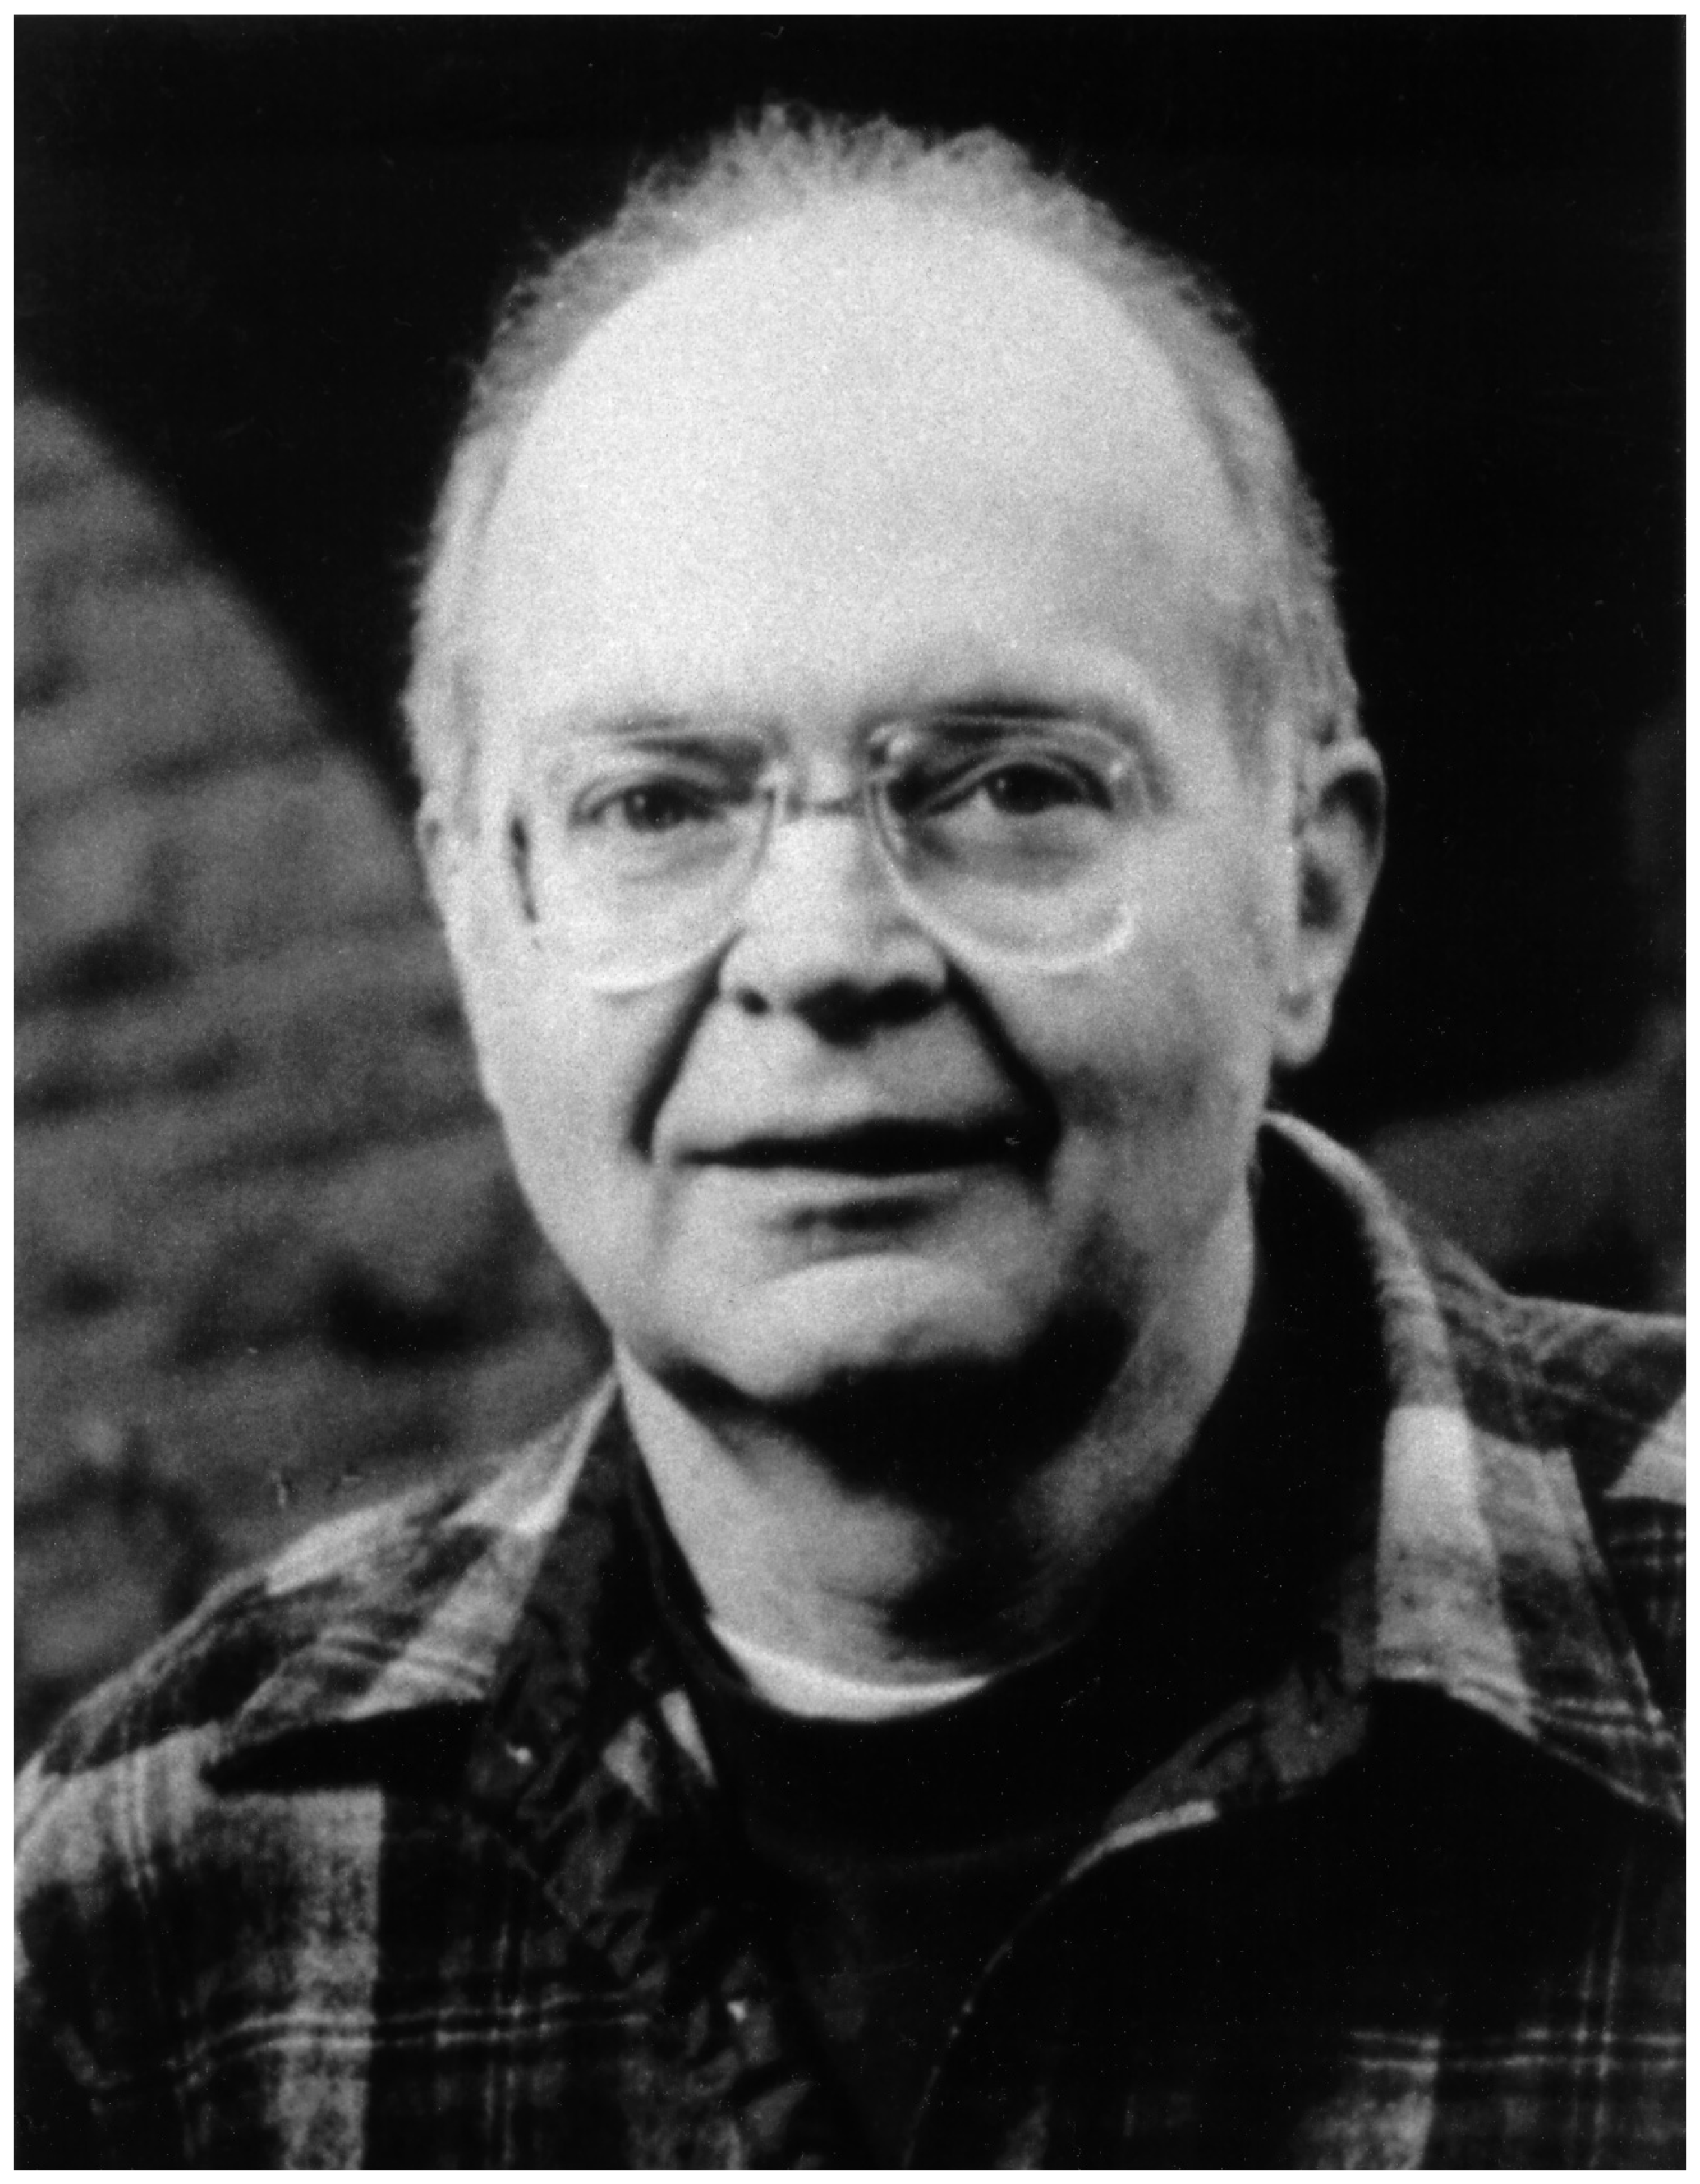
\includegraphics[height=2cm]{don-hires}}
  \caption{包含子图形的大图形}
  \label{fig:big1}
\end{figure}

培育英才万万千,建设祖国锦绣河山,华师儿女奋勇当先,珠江滚滚红绵艳~,岭南大地草木
春,改革开放阳光好,华师园里花烂漫。

艰苦奋斗众志坚,严谨治学成风范,求实创新勇开拓,为人师表代代相传,教育改革宏图展,
师范园地好摇篮,培育祖国栋梁材,神圣职责我承担。


下面这个例子显示并排$3\times2$的图片,见图\ref{fig:subfig:3x2}:
\begin{figure}[htb]
\centering
\subfloat[]{\includegraphics[width=.27\textwidth]{typography}} \qquad
\subfloat[]{\includegraphics[width=.27\textwidth]{typography}} \qquad
\subfloat[]{\includegraphics[width=.27\textwidth]{typography}} \qquad
\subfloat[]{\includegraphics[width=.27\textwidth]{typography}} \qquad
\subfloat[]{\includegraphics[width=.27\textwidth]{typography}} \qquad
\subfloat[]{\includegraphics[width=.27\textwidth]{typography}}
\caption{并排图片}
\label{fig:subfig:3x2}
\end{figure}

要注意,\texttt{qquad}相当于\verb|\hspace{2em}|,也就是2个字符的宽度,约0.08倍页宽,
图片宽度设定为0.27倍页宽是合适的;在该环境中,尽量不要手动换行。

向前向前向前向前,华师儿女永远向前!

如果要把编号的两个图形并排,那么小页就非常有用了:
\begin{figure}[htb]
\begin{minipage}{0.48\textwidth}
  \centering
  \includegraphics[height=4cm]{building.jpg}
  \caption{并排第一个图}
  \label{fig:parallel1}
\end{minipage}\hfill
\begin{minipage}{0.48\textwidth}
  \centering
  \includegraphics[height=4cm]{cat.jpg}
  \caption{并排第二个图}
  \label{fig:parallel2}
\end{minipage}
\end{figure}

\section{公式定理}
\label{sec:equation}
贝叶斯公式如式~(\ref{equ:chap1:bayes}),其中 $p(y|\mathbf{x})$ 为后验;
$p(\mathbf{x})$ 为先验;分母 $p(\mathbf{x})$ 为归一化因子。
\begin{equation}
\label{equ:chap1:bayes}
p(y|\mathbf{x}) = \frac{p(\mathbf{x},y)}{p(\mathbf{x})}=
\frac{p(\mathbf{x}|y)p(y)}{p(\mathbf{x})} 
\end{equation}

论文里面公式越多,\TeX{} 就越 happy。再看一个 \textsf{amsmath} 的例子:
\newcommand{\envert}[1]{\left\lvert#1\right\rvert} 
\begin{equation}\label{detK2}
\det\mathbf{K}(t=1,t_1,\dots,t_n)=\sum_{I\in\mathbf{n}}(-1)^{\envert{I}}
\prod_{i\in I}t_i\prod_{j\in I}(D_j+\lambda_jt_j)\det\mathbf{A}
^{(\lambda)}(\overline{I}|\overline{I})=0.
\end{equation} 

大家在写公式的时候一定要好好看 \textsf{amsmath} 的文档,并参考模板中的用法:
\begin{multline*}%\tag{[b]} % 这个出现在索引中的
\int_a^b\biggl\{\int_a^b[f(x)^2g(y)^2+f(y)^2g(x)^2]
 -2f(x)g(x)f(y)g(y)\,dx\biggr\}\,dy \\
 =\int_a^b\biggl\{g(y)^2\int_a^bf^2+f(y)^2
  \int_a^b g^2-2f(y)g(y)\int_a^b fg\biggr\}\,dy
\end{multline*}

多列公式也是比较常见的情况,比较常用的办法是用align环境实现:

\begin{equation} 
\mathbf{X} = \left(\begin{array}{ccc} 
x_{11} & x_{12} & \ldots \\ 
x_{21} & x_{22} & \ldots \\ 
\vdots & \vdots & \ddots \end{array} \right) 
\end{equation} 

\begin{equation} 
y = \left\{ \begin{array}{ll} 
a & \textrm{if $d>c$}\\ 
b+x & \textrm{in the morning}\\ 
l & \textrm{all day long} 
\end{array} \right. 
\end{equation} 

\begin{equation} 
\left(\begin{array}{c|c} 
1 & 2 \\ 
\hline 3 & 4 \end{array}\right) 
\end{equation}   

\begin{eqnarray}
f(x) & = & \cos x \\ 
f'(x) & = & -\sin x \\ 
\int_{0}^{x} f(y)\,dy & = & \sin x 
\end{eqnarray} 

{\setlength\arraycolsep{2pt} 
\begin{eqnarray} 
\sin x & = & x -\frac{x^{3}}{3!} +\frac{x^{5}}{5!}-{} \nonumber\\ 
	& & {}-\frac{x^{7}}{7!}+{}\cdots 
\end{eqnarray}} 

另外,\texttt{split}环境可能在XeCJK上不能使用,我们测试一下,看\ref{equ:split}:
\begin{equation}\label{equ:split}
\begin{split}
[z^n]C(z) &= [z^n] \biggl[\frac{e^{3/4}}{\sqrt{1-z}} +
e^{-3/4}(1-z)^{1/2} + \frac{e^{-3/4}}{4}(1-z)^{3/2}
+ O\Bigl( (1-z)^{5/2}\Bigr)\biggr] \\
&= \frac{e^{-3/4}}{\sqrt{\pi n}} - \frac{5e^{-3/4}}{8\sqrt{\pi
n^3}} + \frac{e^{-3/4}}{128 \sqrt{\pi n^5}} +
O\biggl(\frac{1}{\sqrt{\pi
n^7}}\biggr)
\end{split}
\end{equation}
\textbf{注意:} 论文模板中为了与xeCJK稳定版本兼容,调校了split命令,代价是不能在inline使用split命令。

\begin{theorem}
  \label{chapTSthm:rayleigh solution}
  假定 $X$ 的二阶矩存在:
  \begin{equation}
         O_R(\textbf{x},F)=\sqrt{\frac{\textbf{u}_1^T\textbf{A}\textbf{u}_1} {\textbf{u}_1^T\textbf{B}\textbf{u}_1}}=\sqrt{\lambda_1},
  \end{equation}
  其中 $\textbf{A}$ 等于 $(\textbf{x}-EX)(\textbf{x}-EX)^T$,\textbf{B} 表示协方差阵 $E(X-EX)(X-EX)^T$,$\lambda_1$
$\textbf{u}_1$ 是 $\lambda_1$对应的特征向量, $\omega,\ve{\omega},\omegaup,\ve{\omegaup}$.
\end{theorem}

\begin{proof}
 上述优化问题显然是一个 Rayleigh 商问题。我们有
  \begin{align}
     O_R(\textbf{x},F)=\sqrt{\frac{\textbf{u}_1^T\textbf{A}\textbf{u}_1} {\textbf{u}_1^T\textbf{B}\textbf{u}_1}}=\sqrt{\lambda_1},
 \end{align}
 其中 $\lambda_1$ 下列广义特征值问题的最大特征值:
$$
\textbf{A}\textbf{z}=\lambda\textbf{B}\textbf{z}, \textbf{z}\neq 0.
$$
 $\textbf{u}_1$ 是 $\lambda_1$对应的特征向量。结论成立。
\end{proof}

\subsection{非回路故障的推理算法}
我们知道,故障诊断的最终目的,是将故障定位到部件,而由于信号-部件依赖矩阵的存在,因此,实质性的工作是找出由故障部件发出异常信号,
不妨称为源异常信号,而如前所述,源异常信号与异常信号依赖矩阵$\mathbf{S_a}$的全零列是存在一一对应的关系的。因此,我们只要获得了$\mathbf{S_a}$的全零列的相关信息,
也就获得了源异常信号的信息,从而能进一步找到故障源。
通过以上分析,我们构造算法\ref{alg53},用于实现非回路故障诊断。

算法\ref{alg53}中,称$\beta$为源异常信号向量,该向量中与源异常信号对应的元素值为1,其它为0;
称$\gamma$为部件状态向量,该向量中非0元素对应的部件为故障部件~,0元素对应的部件为正常部件。
值得一提的是$\beta$和$\beta_a$的区别。$\beta$指出了源异常信号在所有信号中排序的位置,因此其维数与信号总数相同;
而$\beta_a$指出了源异常信号在所有异常信号中排序的位置,因此其维数与异常信号总数相同。如前所述,信号的“排序”是固定的,
这保证了算法在执行中不出现混乱。
\begin{algorithm}[htbp]
  \caption{非回路故障诊断算法}
  \label{alg53}
  \begin{algorithmic}[1]
    \REQUIRE 信号--部件依赖矩阵$\mathbf{A}$,信号依赖矩阵$\mathbf{S}$,信号状态向量$\alpha$
    \ENSURE 部件状态向量$\gamma$
    \STATE $\mathbf{P}\leftarrow\left(<\alpha>\right)$
    \STATE $\mathbf{S_{a}}\leftarrow\mathbf{P^T}\mathbf{S}\mathbf{P}$
    \FOR{$i=1$ to $S_a$的阶数$m$}
    \STATE $s_i\leftarrow s_i$的第$i$个行向量
    \ENDFOR
    \STATE $\beta_a\leftarrow\lnot \left(s_1\lor s_2\lor \cdots\lor s_m\right)^T$
    \STATE $\beta\leftarrow\mathbf{P}\beta_a$
    \STATE $\gamma\leftarrow\mathbf{A}\beta$
  \end{algorithmic}
\end{algorithm}
\subsubsection{第一类故障回路的推理算法}
第一类故障回路推理与非回路故障推理是算法基本相同,稍微不同的是$\beta_a$的计算。因为第一类故障回路中的信号全部可能是源异常信号,因此我们不必计算
$\beta_a=\lnot \left(\left[s_1\lor s_2\lor \cdots\lor s_m\right]^T\right)$,而直接取$\beta_a=\underbrace{\left[\begin{array}{cccc}1&1&\cdots&1\end{array}\right]^T}_m$,将$\beta_a$代入
算法\ref{alg53},有
\[\beta=\mathbf{P}\beta_a=\mathbf{P}\underbrace{\left[\begin{array}{cccc}1&1&\cdots&1\end{array}\right]^T}_m=\alpha\]
因此一类故障回路的推理算法变得相当简单,例如算法\ref{alg54}
\begin{algorithm}[htbp]
  \caption{第一类故障回路诊断算法}
  \label{alg54}
  \begin{algorithmic}[1]
    \REQUIRE 信号--部件依赖矩阵$\mathbf{A}$,信号状态向量$\alpha$
    \ENSURE 部件状态向量$\gamma$
    \STATE $\gamma\leftarrow\mathbf{A}\alpha$
  \end{algorithmic}
\end{algorithm}

\section{参考文献}
\label{sec:bib}
当然参考文献可以直接写 bibitem,虽然费点功夫,但是好控制,各种格式可以自己随意改
写,在\scnuthesis{}里面,建议使用JabRef编辑和管理文献,再结合\verb|bstutf8.bst|之后,
对中文的支持也很好。

本模板推荐使用 BIB\TeX,样式文件为 bstutf8.bst,基本符合学校的参考文献格式(如专利
等引用未加详细测试)。看看这个例子,关于书的\upcite{tex, companion},
还有这些\upcite{clzs},关于杂志的\upcite{ELIDRISSI94,
  MELLINGER96, SHELL02},硕士论文\upcite{zhubajie, metamori2004},博士论文
\upcite{shaheshang, FistSystem01},标准文件\upcite{IEEE-1363}~,会议论文\upcite{DPMG},%
技术报告\upcite{NPB2}。中文参考文献\upcite{cnarticle}\textsf{特别注意},需要在\verb|bibitem|中
增加\verb|language|域并设为\verb|zh|,英文此项可不填,之后由\verb|bstutf8|统一处理
(具体就是决定一些文献的显示格式,如等、etc)。
若使用\verb|JabRef|,则选择\textsf{Options}$\rightarrow$\textsf{Set Up General Fields},
在\verb|General:|后加入\verb|language|就可以了。

有时候不想要上标,那么可以这样 \cite{shaheshang},这个非常重要。

\section{代码高亮}
有些时候我们需要在论文中引入一段代码,用来衬托正文的内容,或者体现关键思路的实现。
在模板中,统一使用\texttt{listings}宏包,并且设置了基本的内容格式,并建议用户只
使用三个接口,分别控制:编程语言,行号以及边框。简洁达意即可,下面分别举例说明。

首先是设定语言,来一个C的,使用的是默认设置:
\begin{lstlisting}[language=C]
void sort(int arr[], int beg, int end)
{
  if (end > beg + 1)
  {
    int piv = arr[beg], l = beg + 1, r = end;
    while (l < r)
    {
      if (arr[l] <= piv)
        l++;
      else
        swap(&arr[l], &arr[--r]);
    }
    swap(&arr[--l], &arr[beg]);
    sort(arr, beg, l);
    sort(arr, r, end);
  }
}
\end{lstlisting}

当我们需要高亮Java代码,不需要行号,不需要边框时,可以:
\begin{lstlisting}[language=Java,numbers=none,frame=none]
// A program to display the message
// "Hello World!" on standard output

public class HelloWorld {
 
   public static void main(String[] args) {
      System.out.println("Hello World!");
   }
      
}   // end of class HelloWorld
\end{lstlisting}

细心的用户可能发现,行号被放在了正文框之外,事实上这样是比较美观的,如果有些用户希望在正文框架之内布置所有内容,
可以:
\begin{lstlisting}[language=perl,xleftmargin=2em,framexleftmargin=1.5em]
#!/usr/bin/perl
print "Hello, world!\n";
\end{lstlisting}

好了,就这么多,\texttt{listings}宏包的功能很强大也很复杂,如果需要自己定制,可以
查看其手册,耐心阅读总会找到答案。\textbf{注意:} 当前中文注释的处理还不是很完善,
对于注释请妥善处理。在本模板中,推荐算法环境或者去掉中文的listings代码环境。如果
需要包含中文注释,不要求代码高亮~,就用\texttt{code}环境,这个环境是Verbatim的定制
版,调用的fancyvbr宏包,用户可在myscnu.sty中修改。

\begin{code}
public class HelloWorld {
   public static void main(String[] args) {
      System.out.println("Hello World!");
   }
}   // 世界,你好!
\end{code}

\section{中文习惯}
\label{sec:chinese}

对于itermize过大的行间距,用户可以使用compactitem环境来替代,但是模板中不进行默认替代,
因为只有用户真正发现列表不好看才会找到这里。

对于中文双引号,可以直接使用全角的\verb|“|和\verb|”|。但是英文则不行!英文的引
号用法请自行Google,或者阅读我的
\href{https://dl.dropbox.com/u/49734213/LaTeX%E6%9C%AD%E8%AE%B0.pdf}{\LaTeX{}}札
记。

中文破折号为一个两个字宽垂直居中的直线,输入法直接得到的破折号没有垂直居中(——),
这看起来不舒服。所以模板中定义了一个破折号的命令 \verb|\pozhehao|,请看:

艰苦奋斗、严谨治学、求实创新、为人师表\hfill \pozhehao{}华南师范大学校训
%!TEX root = ../thesis.tex
\chapter{结论}
\label{chap:conclusion}

如来道:“圣僧,汝前世原是我之二徒,名唤金蝉子。因为汝不听说法,轻慢
我之大教,故贬汝之真灵,转生东土。今喜皈依,秉我迦持,又乘吾教,取去真经,
甚有功果,加升大职正果,汝为旃檀功德佛。孙悟空,汝因大闹天宫,吾以甚深法
力,压在五行山下,幸天灾满足,归于释教;且喜汝隐恶扬善,在途中炼魔降怪有
功,全终全始,加升大职正果,汝为斗战胜佛。猪悟能,汝本天河水神,天蓬元帅。
为汝蟠桃会上酗酒戏了仙娥,贬汝下界投胎,身如畜类。幸汝记爱人身,在福陵山
云栈洞造孽,喜归大教,入吾沙门,保圣僧在路,却又有顽心,色情未泯。因汝挑
担有功,加升汝职正果,做净坛使者。”八戒口中嚷道:“他们都成佛,如何把我
做个净坛使者?”如来道:“因汝口壮身慵,食肠宽大。盖天下四大部洲,瞻仰吾
教者甚多,凡诸佛事,教汝净坛,乃是个有受用的品级。如何不好——沙悟净,汝
本是卷帘大将,先因蟠桃会上打碎玻璃盏,贬汝下界,汝落于流沙河,伤生吃人造
孽,幸皈吾教,诚敬迦持,保护圣僧,登山牵马有功,加升大职正果,为金身罗汉。”
又叫那白马:“汝本是西洋大海广晋龙王之子。因汝违逆父命,犯了不孝之罪,幸
得皈身皈法,皈我沙门,每日家亏你驮负圣僧来西,又亏你驮负圣经去东,亦有功
者,加升汝职正果,为八部天龙。”

因此:

\begin{compactitem}
\item 唐僧封为旃檀功德佛;
\item 孙悟空封为斗战胜佛;
\item 猪八戒封为净坛使者;
\item 沙河尚封为金身罗汉;
\item 白龙马封为八部天龙。
\item 华师是个好学校。
\end{compactitem}




\cleardoublepage
\renewcommand{\chapterlabel}{\bibname} % 设置页眉
\bibliographystyle{bstutf8}
\bibliography{ref/refs}

\appendix
\backmatter

%%% Local Variables:
%%% mode: latex
%%% TeX-master: "../main"
%%% End:

\section{外文资料原文}
\label{cha:engorg}
\subsection[First Principles]{first principles}

\subsubsection{Typography exists to honor content.}

Like oratory, music, dance, calligraphy -- like anything that lends its grace to language -- typography is an art that can be deliberately misused. It is a craft by which the meanings of a text (or its absence of meaning) can be clarified, honored and shared, or knowingly disguised.

In a world rife with unsolicited messages, typography must often draw attention to itself before it will be read. Yet in order to be read, it must relinquish the attention it has drawn. Typography with anything to say therefore aspires to a kind of statuesque transparency. Its other traditional role is durability: not immunity to change, but a clear superiority to fashion. Typography at its best is a visual form of language linking timelessness and time.

One of the principles of durable typography is always legibility; another is something more than legibility: some earned or unearned interest that gives its living energy to the page. It takes various forms and goes by various names, including serenity, liveliness, grace and joy.

These principles apply, in different ways, to the typography of business cards, instruction sheets and postage stamps, as well as to editions of religious scriptures, literary classics and other books that aspire to join their ranks. Within limits, the same principles apply even to stock market reports, airline schedules, milk cartons, classified ads. But laughter, grace and joy, like legibility itself, all feed on meaning, which the writer, the words and the subject, not the typographer, must generally provide.

In 1770, a bill was introduced in the English Parliament with the following provisions:
\begin{quote}$\ldots$ all women of whatever age, rank, profession, or degree, whether virgins, maids, or widows, that shall $\ldots$ impose upon, seduce, and betray into matrimony, any of His Majesty's subjects, by the scents, paints, cosmetic washes, artificial teeth, false hair, Spanish wool, iron stays, hoops, high heeled shoes {\rm [}or{\rm ]} bolstered hips shall incur the pen\-alty of the law in force against witchcraft $\ldots$ and $\ldots$ the marriage, upon conviction, shall stand null and void.
\end{quote}
The function of typography, as I understand it, is neither to further the power of witches nor to bolster the defenses of those, like this unfortunate parliamentarian, who live in terror of being tempted and deceived. The satisfactions of the craft come from elucidating, and perhaps even ennobling, the text, not from deluding the unwary reader by applying scents, paints and iron stays to empty prose. But humble texts, such as classified ads or the telephone directory, may profit as much as anything else from a good typographical bath and a change of clothes. And many a book, like many a warrior or dancer or priest of either sex, may look well with some paint on its face, or indeed with a bone in its nose.

\subsubsection{Letters have a life and dignity of their own.}

Letterforms that honor and elucidate what humans see and say deserve to be honored in their turn. Well-chosen words deserve well-chosen letters; these in their turn deserve to be set with affection, intelligence, knowledge and skill. Typography is a link, and it ought, as a matter of honor, courtesy and pure delight, to be as strong as the others in the chain.

Writing begins with the making of footprints, the leaving of sighs. Like speaking, it is a perfectly natural act which humans have carried to complex extremes. The typographer's task has always been to add a somewhat unnatural edge, a protective shell of artificial order, to the power of the writing hand. The tools have altered over the centuries, and the exact degree of unnaturalness desired has varied from place to place and time to time, but the character of the essential transformation between manuscript and type has scarcely changed.

The original purpose of type was simply copying. The job of the typographer was to imitate the scribal hand in a form that permitted exact and fast replication. Dozens, then hundreds, then thousands of copies were printed in less time than a scribe would need to finish one. This excuse for setting texts in type has disappeared. In the age of photolithography, digital scanning and offset printing, it is as easy to print directly from handwritten copy as from text that is typographically composed. Yet the typographer's task has little changed. It is still to give the illusion of superhuman speed and stamina -- and of superhuman patience and precision~-- to the writing hand.

Typography is just that: idealized writing. Writers themselves now rarely have the calligraphic skill of earlier scribes, but they evoke countless versions of ideal script by their varying voices and literary styles. To these blind and often invisible visions, the typographer must respond in visible terms.

\appendixsection{其它附录}
\appendixitem{说明}
其它附录的内容可以放到这里,当然如果你愿意,可
以把这部分也放到独立的文件中,然后将其 \verb|\input| 到主文件中。


\cleardoublepage
\renewcommand{\chapterlabel}{\ackname} % 设置致谢参考文献的页眉
%%% Local Variables:
%%% mode: latex
%%% TeX-master: "../main"
%%% End:
%!TEX root = ../thesis.tex

\begin{ack}

  首先要感谢党,感谢国家!
  
  这份模板的制作首先得到了我的导师计算机学院李兴民教授,以及计算机学院陈寅副教授的
  热心支持,衷心感谢他们的教诲和指导意见!

  除此之外,还要感谢计算机学院的卓雄辉书记、雷蕾副书记、汤庸院长、单志龙副院长、王
  立斌副教授等,感谢他们对我的鼓励和帮助。

  在做这个模板的时候也获得了其他高校的\TeX{}er们的帮助,尤其是国防科大
  的\nudtpaper{}和清华大学的\thuthesis{},如果没有这些前辈们的工作,这份模板也不
  可能这么快出来和大家见面。另外,感谢戴高远,潘嘉昕,高有等同学为这个模板提供了
  很多宝贵的素材和建议,感谢周晓倩同学和莫城为同学参与模板的测试工作。

  感谢以上所有人的努力付出,希望\scnuthesis{}能够在未来的日子里成
  为\textit{SCNUer}们的毕业论文好帮手,帮助大家完成格式规范、排版精美的论文!

\end{ack}


\cleardoublepage
\renewcommand{\chapterlabel}{\resumename} % 设置作者个人成果的页眉
\input{data/resume}

\end{document}
